% Beamer slide template prepared by Tom Clark <tom.clark@op.ac.nz>
% Otago Polytechnic
% Dec 2012

\documentclass[10pt]{beamer}
\usetheme{Dunedin}
\usepackage{graphicx}
\usepackage{fancyvrb}
\usepackage{hyperref}

\newcommand\codeHighlight[1]{\textcolor[rgb]{1,0,0}{\textbf{#1}}}

\title{Xen Networking}

\author[I720]{Virtualisation}
\institute[Otago Polytechnic]{
  Otago Polytechnic \\
  Dunedin, New Zealand \\
}
\date{}
\begin{document}



%----------- titlepage ----------------------------------------------%
\begin{frame}[plain]
  \titlepage
\end{frame}


\begin{frame}
  
  In our guest configuration files, we have been using the following line to configure guest networking:
  
  \vspace{5mm}
  
  \texttt{ vif =['']}
  
  \vspace{5mm}
  What does it mean?
  
  \end{frame}
  

\begin{frame}[fragile]
  \frametitle{Default network settings}
  
   It means to use the defaults. But what are those?
   
  \vspace{5mm}
  Default network settings are defined in \texttt{/etc/xen/xl.conf}. The relevant ones right now are
  
  \vspace{5mm}
  

\begin{verbatim}
 vif.default.script="vif-bridge"
 vif.default.bridge="xenbr0"
 vif.default.backend="0"
\end{verbatim}

\vspace{5mm}
To see what these mean, we need a little background.
\end{frame}

\begin{frame}
  \frametitle{Three networking options}
  
  \begin{itemize}
    \item Bridged networking
    \item Routing
    \item NAT
  \end{itemize}
  
  Bridged networking is the default.
  
  \vspace{5mm}
  Note than none of these networking schemes are provided by Xen. They are provided through
  the underlying capabilities of the Dom0 operating system.
  
  \end{frame}

\begin{frame}

    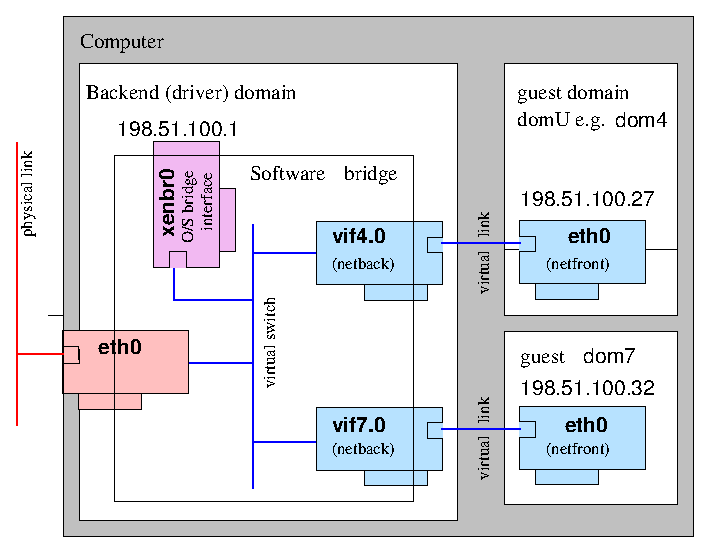
\includegraphics[width=\linewidth]{network-bridge}
\end{frame}


\begin{frame}
  \frametitle{How did we set this up?}
 
 Recall that when we were installing Xen and setting up Dom0, we
 
    \begin{itemize}
    \item Installed \texttt{bridge-utils};
    \item Configured the \texttt{xenbr0} interface;
    \item Removed the DHCP configuration from the \texttt{eth0} interface.
  \end{itemize}
\end{frame}

\begin{frame}
  \frametitle{How did we set this up?}
 
 Then, every time we create a guest, the script specified by 
 \texttt{vif.default.script} is run. This
 
    \begin{itemize}
    \item Sets up the \texttt{vif.X.0} interface on Dom0;
    \item Configures the \texttt{eth0} interface on the guest;
    \item Adds any needed bridging configuration.
  \end{itemize}
\end{frame}

\begin{frame}

    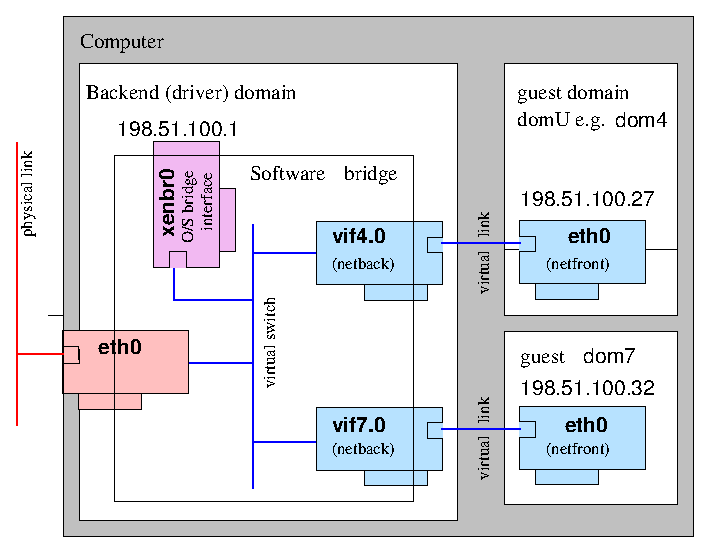
\includegraphics[width=\linewidth]{network-bridge}
\end{frame}

\begin{frame}
  \frametitle{Another bridging option}
  
  Instead of \texttt{bridge-utils}, we can use Open vSwitch to manage bridging on Dom0.
  This provided some more advanced bridging configuration options.
  
  \end{frame}

\begin{frame}
  \frametitle{How do we use routing or nat?}

 
 
    \begin{itemize}
    \item Eliminate the bridged interface and reconfigure Dom0's ethernet interface;
    \item Configure routing/NAT using the capabilities of the Dom0 OS;
    \item Change \texttt{vif.default.script};
    \item Possibly change the guest configuration.
  \end{itemize}
\end{frame}

\begin{frame}[fragile]
  \frametitle{About that guest config}
  
  
   
   \texttt{vif = ['']}
  
  \vspace{5mm}
This is actually Python code. \texttt{vif} is a list of strings. Each one is a comma-separated  set of
key/value pairs. Examples are

\begin{verbatim}
 ''
 'mac=00:16:3E:74:3d:76'
 'script=custom-bridging,bridge=xenbridge2'
 'ip=192.168.10.44'
\end{verbatim}

See \texttt{http://xenbits.xen.org/docs/4.2-testing/ \\ misc/xl-network-configuration.html} for more information


\end{frame}

\end{document}
